\section{Introduction}

Reply is a global network of over 150 specialized companies dedicated to helping organizations leverage cutting-edge technologies. 
Our mission is to drive innovation by enabling businesses to adapt to economic shifts and technological advancements, particularly those driven by the internet.
\begin{figure}[H]
    \centering
    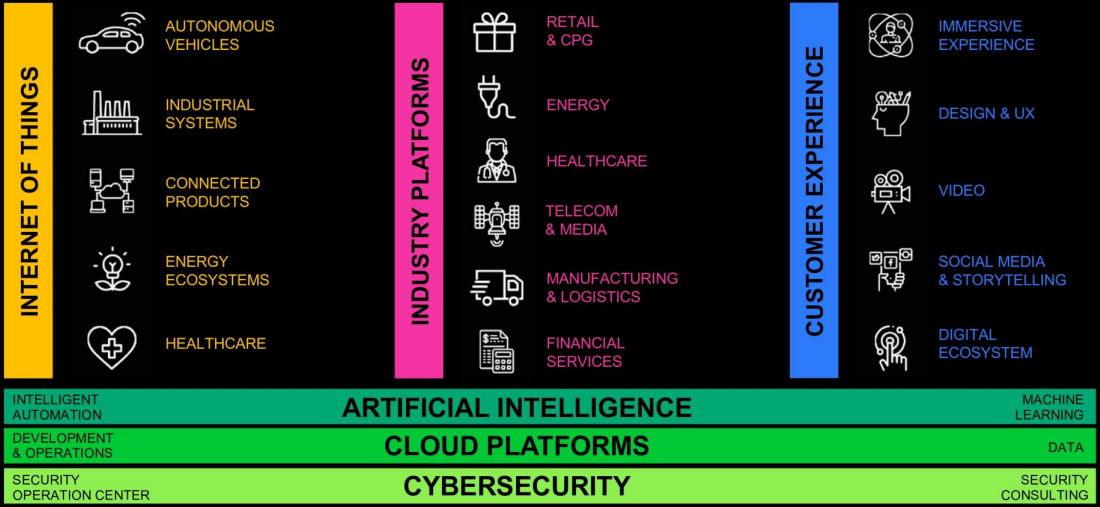
\includegraphics[width=0.5\linewidth]{images/bis2.png}
    \caption{Reply services}
\end{figure}
\noindent Reply provides end-to-end solutions for businesses looking to transform raw data into valuable insights. 
From data collection to advanced analytics, our approach ensures that companies can harness the full potential of their data.




\subsection{Data}
Data has become the foundation of decision-making, shaping industries and redefining business strategies. 
The journey of data-driven innovation can be divided into several key phases:

\begin{chronology}[5]{2010}{2025}{0.9\textwidth}
    \event[2012]{2015}{Big data}
    \event[2015]{2018}{Machine Learning}
    \event[2014]{2017}{Cloud computing}
    \event[2017]{2025}{Generative AI}
\end{chronology}

\paragraph*{Big data} 
Big data refers to the exponential growth of structured and unstructured data generated daily. 
It brought new challenges in storage, management, and analysis but also unlocked vast opportunities for business intelligence.
\renewcommand*{\arraystretch}{1.5}
\begin{table}[H]
    \centering
    \begin{tabular}{|l|l|}
    \hline
    \textbf{Technology} & Hadoop, Hive, Impala, Cloudera                                           \\ \hline
    \textbf{Key impact} & Data-driven decision-making, process optimization, competitive advantage \\ \hline
    \end{tabular}
\end{table}
\renewcommand*{\arraystretch}{1}

\paragraph*{Machine Learning}
Machine Learning marked the next stage of data evolution, enabling computers to learn patterns and make decisions without explicit programming. 
Machine Learning applications expanded rapidly, offering predictive insights and automation capabilities.
\renewcommand*{\arraystretch}{1.5}
\begin{table}[H]
    \centering
    \begin{tabular}{|l|l|}
    \hline
    \textbf{Technology} & Neural Networks, Deep Learning, Reinforcement Learning, Clustering                                  \\ \hline
    \textbf{Key impact} & Advanced automation, improved predictions, enhanced decision-making \\ \hline
    \end{tabular}
\end{table}
\renewcommand*{\arraystretch}{1}

\paragraph*{Cloud Computing}
Cloud computing revolutionized data storage and processing by providing scalable, cost-effective solutions over the internet. 
Businesses gained access to flexible computing power, reducing infrastructure constraints.
\renewcommand*{\arraystretch}{1.5}
\begin{table}[H]
    \centering
    \begin{tabular}{|l|l|}
    \hline
    \textbf{Technology} & AWS, Google Cloud Platform, Microsoft Azure                                 \\ \hline
    \textbf{Key impact} & Scalability, cost reduction, innovation acceleration \\ \hline
    \end{tabular}
\end{table}
\renewcommand*{\arraystretch}{1}

\paragraph*{Generative Artificial Intteligence}
Generative AI represents the latest frontier, where AI systems exhibit human-like understanding, learning, and application of knowledge across diverse domains.
Its potential is reshaping industries and redefining human-technology interaction.
\renewcommand*{\arraystretch}{1.5}
\begin{table}[H]
    \centering
    \begin{tabular}{|l|l|}
    \hline
    \textbf{Technology} & Large Language Models, synthetic data, Retrieval-Augmented Generation                                 \\ \hline
    \textbf{Key impact} & Creative automation, enhanced productivity, AI-driven decision making \\ \hline
    \end{tabular}
\end{table}
\renewcommand*{\arraystretch}{1}

\begin{figure}[H]
    \centering
    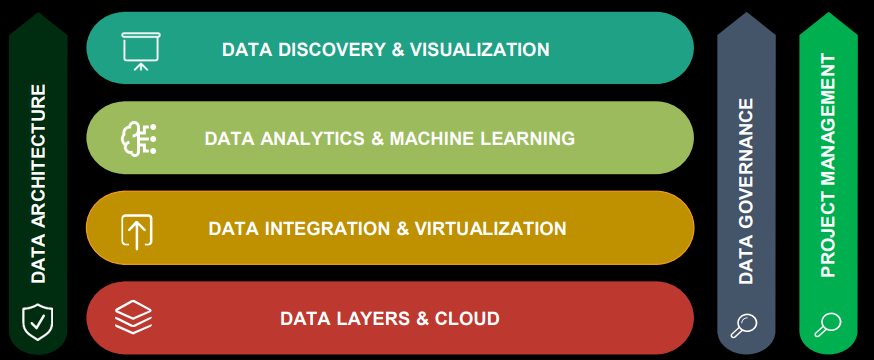
\includegraphics[width=0.5\linewidth]{images/bis3.png}
    \caption{Data framework}
\end{figure}


\subsection{Data job roles}

\paragraph*{Data and Cloud architect}
Data architects design comprehensive data infrastructures based on business objectives, ensuring seamless data integration and optimal storage solutions. 
Cloud Architects specialize in designing scalable, cloud-based architectures to support modern data needs.

\paragraph*{Data engineer}
Data engineers build and maintain the systems required for collecting, processing, and storing data. 
They design ETL pipelines, work with big data technologies, and ensure that raw data is transformed into a usable format.

\paragraph*{Data analyst}
Data analysts interpret and analyze data to provide actionable insights. 
They clean datasets, perform statistical analysis, and create visualizations to support business strategies and decision-making.

\paragraph*{Data scientist}
Data scientists develop machine learning models and apply advanced analytics to uncover patterns and predictions from complex datasets. 
They work with programming languages like Python and utilize AI-driven techniques for deeper insights.

\paragraph*{Data privacy and security specialist}
Data privacy officers ensure compliance with data protection regulations (e.g., GDPR), while security officers implement safeguards to protect organizational data from cyber threats and breaches.